%-----------------------------------------------------------------------------------------------
\chapter{Markers}\label{sect:marker}
%-----------------------------------------------------------------------------------------------

One of the goals of this project was to design a fiducial marker with advantageous properties for use in pose estimation.
In a typical scenario the marker may be seen from largely varying viewpoints, therefore it has to have some level of scale invariability.
If the observer is far from the marker, the smaller details may be lost due to the limited resolution of the camera.
If the same observer moves closer to the marker, it may fill the whole field of view and some features may even slip off the image.
This leads to another feature the marker needs to have: redundancy.
If the observer gets too close to the marker or some obstacle partially blocks the view, the localisation still needs to provide usable results.

The intended use of the markers is spatial localisation and pose estimation.
In other words: approximating the observers 3D coordinates ($x, y, z$) and orientation ($\phi, \theta, \psi$) with respect to the marker.
It is supposed that the observer uses a single camera system for navigation (e.g. smartphone or robotic application with limited resources).
This means the marker needs at least 6 degree of freedom.

To sum up the above discussed specifications, a suitable marker would have to:
\begin{itemize}
	\item have at least 6 DOF
	\item be (to some degree) scale invariant
	\item have redundancy
\end{itemize}

In the following sections will be a recommendation for a marker conforming for the listed specifications.
It is based on 3 connected line segments forming a quad with one missing side.
The whole marker is built from quads with different side lengths and angles.

%-----------------------------------------------------------------------------------------------
\section{Quad}
%-----------------------------------------------------------------------------------------------

A marker is put together from quads.
Figure \figref{exampleQuads} shows two examples.
One side of the quads is left out: they are put together from three joint line segments.
The middle segment, with two adjoining lines, will be referred to as the 'base' of the quad.
The outer segments are going to be called 'arms'.

\begin{figure}
	\begin{subfigure}{0.5\textwidth}
		\centering
		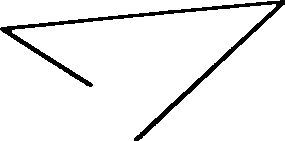
\includegraphics[width=0.75\textwidth]{figures/quad1.png}
	\end{subfigure}
	\begin{subfigure}{0.5\textwidth}
		\centering
		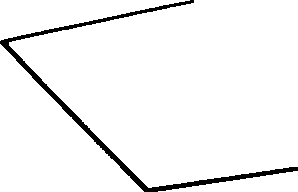
\includegraphics[width=0.75\textwidth]{figures/quad2.png}
	\end{subfigure}
	\caption{Example for different quads}
	\label{fig:exampleQuads}
\end{figure}

A quad has 6 degrees of freedom.
There are 3 independent distance parameters: the length of the base and the two arm segments.
There are also 3 unrelated angle parameters: the angles between each arm and the base, and the orientation of the quad.

\begin{figure}[ht]
	\centering
	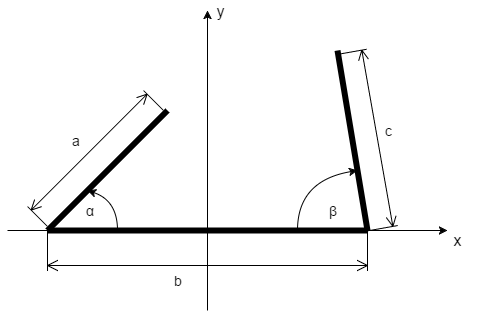
\includegraphics[width=0.75\textwidth]{figures/quad_params.png}
	\caption{Quad parameters}
	\label{fig:quadParams}
\end{figure}

Figure \figref{quadParams} shows the free parameters of a quad (the orientation is not shown on the image).
The following notation is used:
\begin{itemize}
	\item[a]: The length of one arm
	\item[b]: The length of the base
	\item[c]: The length of the other arm
	\item[$\alpha$]: The angle between one arm and the base
	\item[$\beta$]: The angle between the other arm and the base
	\item[$\gamma$]: The angle with which the whole quad is rotated
\end{itemize}
For the sake of simplicity, figure \figref{quadParams} does not show the rotation with $\gamma$.
The quad would be rotated around the origin of it's coordinate system.

The values of the length parameters are given in pixels, although they can be expressed in any unit of distance.
The angles can be given is degrees or radians (in the implementation degrees are used for easier human readability).

\begin{equation}
	a\in(0 , a_{max}]
	\label{eq:aRange}
\end{equation}
\begin{equation}
	b\in(0 , b_{max}]
	\label{eq:bRange}
\end{equation}
\begin{equation}
	c\in(0 , c_{max}]
	\label{eq:cRange}
\end{equation}
\begin{equation}
	\alpha\in(0 , 180^\circ)
	\label{eq:alphaRange}
\end{equation}
\begin{equation}
	\beta\in(0 , 180^\circ)
	\label{eq:betaRange}
\end{equation}
\begin{equation}
	\gamma\in[0 , 360^\circ)
	\label{eq:gammaRange}
\end{equation}

Equations \eqref{aRange} through \eqref{gammaRange} specify the range of each parameter.
The maximum of the distance parameters are set by the space left on the image for the given marker, there is no theoretical limit for them.
There is also no constraint for the resolution of the parameters.
From the applications point of view, there are quads with continuous\footnote{That is, only limited by the computational precision} and discrete parameter spaces.

%-----------------------------------------------------------------------------------------------
\subsection{Quad representation}
%-----------------------------------------------------------------------------------------------

There are several ways to represent quads, each with different advantageous properties.
For this work multiple considerations were made in that regard.
The most straightforward is to simply store the above mentioned parameters.
This is simple and easy for human reading, which is great help in the development process.

A step forward from this is to norm the $a,b$ and $c$ parameter of the quad with the base segment's length.
Then the following parameters are used:
\begin{itemize}
	\item[s]: marker size, the same as the base length
	\item[$m_a$]: 'a' multiplier. $m_a = a/b$
	\item[$m_c$]: 'c' multiplier. $m_c = c/b$
\end{itemize}
The $\alpha,\beta,\gamma$ angle parameters are not changed.
This gives a scale or size parameter for the quad, which is useful for marker generation.
These two representations are good for development and marker generation, but not so much for calculations.

A third option is to store the endpoints of the line segments.
It requires the storage of 4 points: two endpoints ($E_1,E_2$) and two inner points ($I_1,I_2$).
Equations \eqref{innerPoint1Def} through \eqref{endPoint2Def} define the points' coordinates before rotating with $\gamma$, using figure \figref{quadParams}'s notation.
\begin{equation}
	\label{eq:innerPoint1Def}
	I_1' = (-\frac{b}{2}, 0)
\end{equation}
\begin{equation}
	\label{eq:innerPoint2Def}
	I_2' = (\frac{b}{2}, 0)
\end{equation}
\begin{equation}
	\label{eq:endPoint1Def}
	E_1' = (-\frac{b}{2} + b*cos(\alpha),a*sin(\alpha))
\end{equation}
\begin{equation}
	\label{eq:endPoint2Def}
	E_2' = (\frac{b}{2} - c*cos(\beta),c*sin(\beta))
\end{equation}
\begin{equation}
	\label{eq:rotMatrix}
	Rot(\gamma) = \left( \begin{array}{cc}
	cos(\gamma) & -sin(\gamma)  \\
	sin(\gamma) & cos(\gamma)  \end{array} \right)
\end{equation}
The point $E_1,E_2,I_1,I_2$ can be obtained from $E_1',E_2',I_1',I_2'$ by a multiplication with the rotational matrix $Rot(\gamma)$.

That method is redundant for storage: it uses 8 parameters instead of 6.
However this poses no practical problem in the scope of the project.
The one outstanding benefit of this method is it's efficiency in calculations.
Because it is based on points in a Euclidean space, linear algebraic methods (matrix multiplications) can be used for calculating the projective transformations.

In this project the second and the third options are used.
The first, naive method is omitted because it has no considerable advantage over the other two.
The second method, using the size, multiplier and angle parameters is used in marker generation.
The third is used during the calculations and the recognition process.

%-----------------------------------------------------------------------------------------------
\section{Marker}
%-----------------------------------------------------------------------------------------------

Quads are 6 DOF shapes: in theory it would be enough to use only one of them for localisation and pose estimation.
However that method would have very low error tolerance and questionable accuracy even in a best case scenario.
To comply with the specifications written in the beginning of this chapter, the markers are put together from multiple quads.
By placing quads with different orientations and sizes the error tolerance and accuracy can be greatly improved.

An intrinsic positive quality of using multiple quads with varying sizes is the scale invariance.
As mentioned, even a single quad is sufficient for the task at hand.
If the smaller quads become unrecognisable because of the low resolution or too large distance, a successful measurement is still possible.
The same is true on the other end of the spectrum: if the observer is too close to the marker and the larger ones leave the field of view, the position and orientation can be calculated from the smaller quads.

Figure \figref{rqimExample} shows an example for a marker.
It is generated with the simple algorithm described in the next section, and is not optimal in many ways.
Nonetheless it is functional, even if only a fraction of the quads are registered for the measurement.
\begin{figure}[ht]
	\centering
	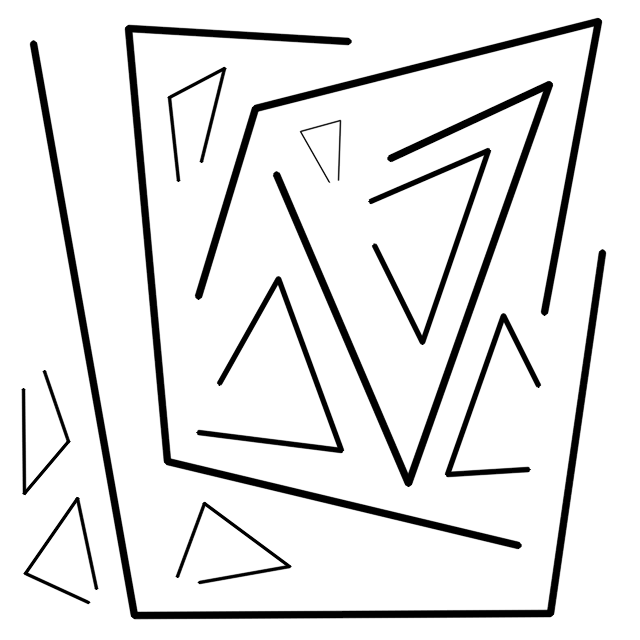
\includegraphics[width=0.75\textwidth]{figures/RQIM_1.png}
	\caption{An example for a marker}
	\label{fig:rqimExample}
\end{figure}

The markers are going to be referred to as RQIM, which means Random Quad Image Marker.
As the name suggests, the quads are randomly generated and placed on the markers.

Unless otherwise specified, RQIMs use quads with continuous parameter spaces.
In this chapter there will also be a small introduction to discrete parameter markers and their potential applications.

%-----------------------------------------------------------------------------------------------
\subsection{Marker generation}
%-----------------------------------------------------------------------------------------------

In the current state of the project, markers are randomly generated using a simple algorithm.
The generator routine receives the number of quads to be used in the current RQIM.
The core concept is to create the desired number of random quads and place them on the image.

Let the number of quads to generate be $n$.
First, the quad sizes are picked.
There is an upper and a lower limit for them, given in percent of the image size.
The generated sizes follow an exponential distribution:
\begin{equation}
	s = e^{-x*f}
\end{equation}
Where $s$ is the quad size, $x$ is random number between 0 and 1 with uniform distribution, and $f$ is a scale factor.
Then the $n$ sizes are ordered in descending order.

After the scale factors are picked, the whole quads are generated by the following method.
A random quad is created with the first (the largest) scale and placed on the image.
Then another quad is created with the next largest size.
After every new quad a check is performed whether or not it can be placed on the marker.
If it cannot, then a new quad is generated with the same scale factor until it can be placed or the algorithm reached the limit of retries.

With this simple logic $n$ quads are placed on the RQIM and the creation process is finished.
Below is the pseudo-code of the algorithm.

\begin{lstlisting}
n_max = number of quads to create
f = scale factor for exponential distribution
lowlim = lower size limit
uplim = upper size limit
n = 0
while n < n_max
	size = exp(-rand() * f)
	if size > lowlim and size < uplim
		store size
		n = n+1
	endif
end
sort(sizes, descending)
n = 0
while n < n_max
	while quad placed or max tries
		quad = create_random_quad(sizes(n))
		if quad can be placed
			place quad
			n = n+1
		end
	end
end
return marker
\end{lstlisting}

This method is not optimal and is based on trial and error, but it gives usable markers for the development process.

%-----------------------------------------------------------------------------------------------
\subsection{Discrete RQIM}
%-----------------------------------------------------------------------------------------------

There are experiments in progress with discrete parameter space quads.
It may be advantageous to quantize the parameter space in order to decrease the error probability in the pose estimation process.

Quads with finite possible states can be stored using much less resources than their continuous counterpart.
As an example let us take a look at the following quantisation.
\begin{description}
	\item[Angles:] $15^\circ,30^\circ,45^\circ,60^\circ,75^\circ,90^\circ,105^\circ,120^\circ$
	\item[Multipliers:] $0.40, 0.60, 0.80, 1.0, 1.25, 1.50, 1.75, 2.0$
	\item[Orientations:] $0^\circ, 22.5^\circ, 45^\circ, 67.5^\circ \dots 270^\circ, 292.5^\circ, 315^\circ, 337.5^\circ$
	\item[Sizes:] $1, 0.8, 0.6, 0.5, 0.4, 0.3, 0.25, 0.2, 0.1, 0.08, 0.06, 0.05, 0.04, 0.03, 0.025, 0.02$
\end{description}
In this example, there are 8 possible values for the angle parameters, also 8 for the multipliers, 16 for the orientation and also 16 for the sizes.
If the possibilities are stored in a lookup table, it is enough for the quad to store the index at which the value is accessible.
A quad is defined by two angle parameters, two multipliers, an orientation and a size.
The angles (in this case) require at least 3 bits each, the multipliers also.
The orientation and the size need 4 bits each.
That gives a sum of 20 bits per quad, which is significantly less than the space required to store 6 floating point numbers per quad.

This 20 bit word is also usable as an ID for the quad.
It may be possible to code information in these ID-s, so the marker could provide additional information.
This information could be related to and used by the localisation process, or be totally unrelated, general data.
These possibilities have not yet been extensively researched.

The discrete RQIMs are usually less dense than the continuous ones, due to the limited angle possibilities.
This means fewer quads per marker, which leads to decreasing redundancy.
An optimum must be found between the number of quads per RQIM and distance between quads in the parameter space.